\title{Lecture 16\\Methodology for Collaborative Knowledge Base Development}

\begin{frame}
	\titlepage
\end{frame}

\begin{frame}{\\Lecture outline}
	\topline
	\justifying
	Knowledge base developers and their roles. How developers structure an intelligent system (IS) knowledge base. Principles of developer collaboration. Verification and detection of incomplete knowledge.
\end{frame}

\begin{frame}{\\How knowledge base development works}
	\topline
	\justifying
	\vspace{8mm}
	\begin{SCn}
		\begin{figure}[H]
			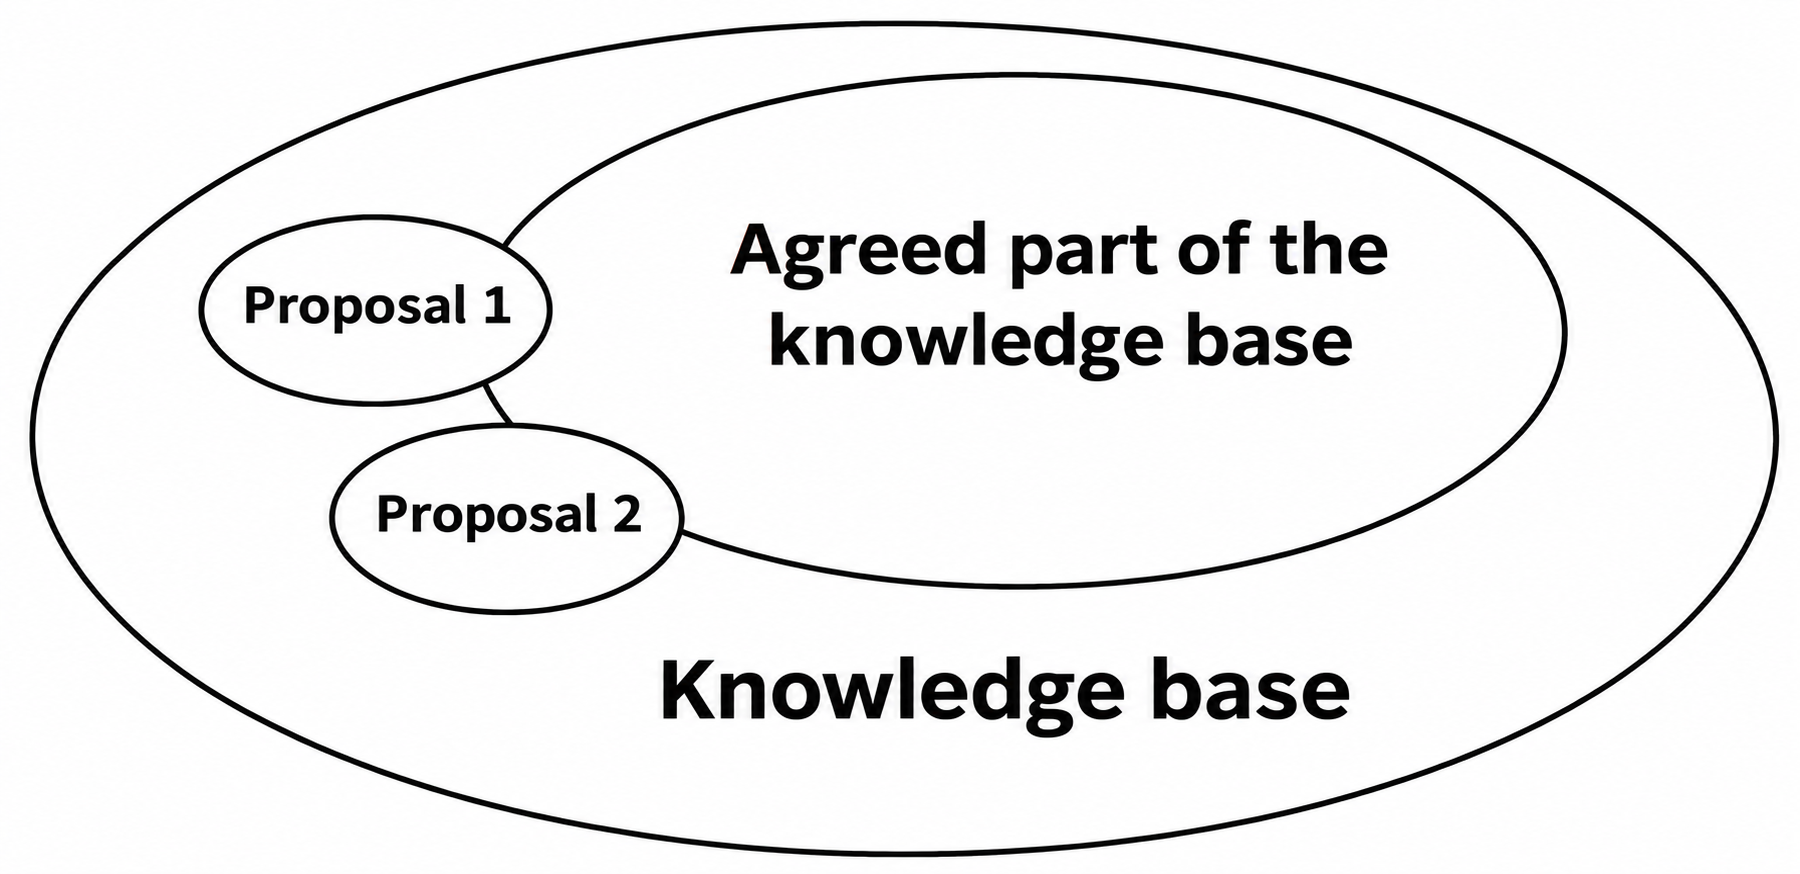
\includegraphics[width=\linewidth,height=0.68\textheight,keepaspectratio]{figures/sd_kb_develop_methods/kb_develop_idea_en.png}
		\end{figure}
	\end{SCn}
\end{frame}

\begin{frame}{\\Unregistered user}
	\topline
	\justifying
	\begin{SCn}
		\scnheader{unregistered user*}
		\scnidtf{binary relation linking an OSTIS system to the sc-element that denotes a person who has not registered with the system}
		\vspace{5mm}

		\textbf{Permissions of an unregistered user}
		\begin{textitemize}
			\item{Read the domain content of the OSTIS knowledge base.}
			\item{Use the OSTIS system in operation mode.}
		\end{textitemize}
	\end{SCn}
\end{frame}

\begin{frame}{\\Registered user}
	\topline
	\justifying
	\begin{SCn}
		\scnheader{registered user*}
		\scnidtf{binary relation linking an OSTIS system to the sc-element that denotes a person who has registered with the system}
		\vspace{10mm}
	\end{SCn}
	\textbf{Permissions of a registered user}
	\begin{textitemize}
		\item{Read the entire knowledge base.}
		\item{Submit proposals for any part of the knowledge base.}
		\item{Use the system in operation or developer mode.}
	\end{textitemize}
\end{frame}

\begin{frame}{\\Knowledge base developer}
	\topline
	\justifying
	\vspace{5mm}
	\begin{SCn}
		\scnheader{developer*}
		\scnsubset{registered user*}
		\scnidtf{binary directed relation linking a project to develop a section of an OSTIS knowledge base (or the entire knowledge base) to the sc-element denoting a person who can carry out project tasks for that section}
	\end{SCn}
	\bigskip
	\textbf{Permissions of a developer}
	\begin{textitemize}
		\item{Read the entire knowledge base.}
		\item{Comment on proposed edits to the knowledge base.}
		\item{Submit proposals for any part of the knowledge base.}
		\item{Use the system in operation or developer mode.}
	\end{textitemize}
\end{frame}

\begin{frame}{\\Developer roles and the administrator}
	\topline
	\justifying
	\begin{SCn}
		\vspace{5mm}
		\scnheader{developer*}
		\begin{scnrelfromset}{partition}
			\scnitem{administrator*}
			\scnitem{manager*}
			\scnitem{expert*}
		\end{scnrelfromset}
		\scnheader{administrator*}
		\scniselement{binary directed relation}
		\scnrelfrom{first domain}{project to develop a section of an OSTIS knowledge base}
		\scnrelfrom{second domain}{sc-element denoting the person who administers that section}
	\end{SCn}
\end{frame}

\begin{frame}{\\Administrator responsibilities}
	\topline
	\justifying
	\begin{SCn}
		\begin{textitemize}
			\item Maintain the integrity and consistency of the entire knowledge base.
			\item Set access levels for other users.
			\item Accept or reject proposals for different parts of the knowledge base and refer them for expert review when needed.
			\item Edit parts of the knowledge base using the appropriate commands. The system automatically records these edits as proposals in the OSTIS system's development history.
		\end{textitemize}
	\end{SCn}
\end{frame}

\begin{frame}{\\Hierarchy of administrators}
	\topline
	\justifying
	\begin{SCn}
		A large knowledge base may require a hierarchy of developers that mirrors the hierarchy of its sections.

		In that case, a lower-level section administrator's approval sends the proposal for review by higher-level administrators before it can be integrated into the section.

		The administrator of the entire knowledge base makes the final decision.
	\end{SCn}
\end{frame}

\begin{frame}{\\Example of an administrator hierarchy}
	\topline
	\justifying
	\vspace{7mm}
	\begin{SCn}
		\begin{figure}[H]
			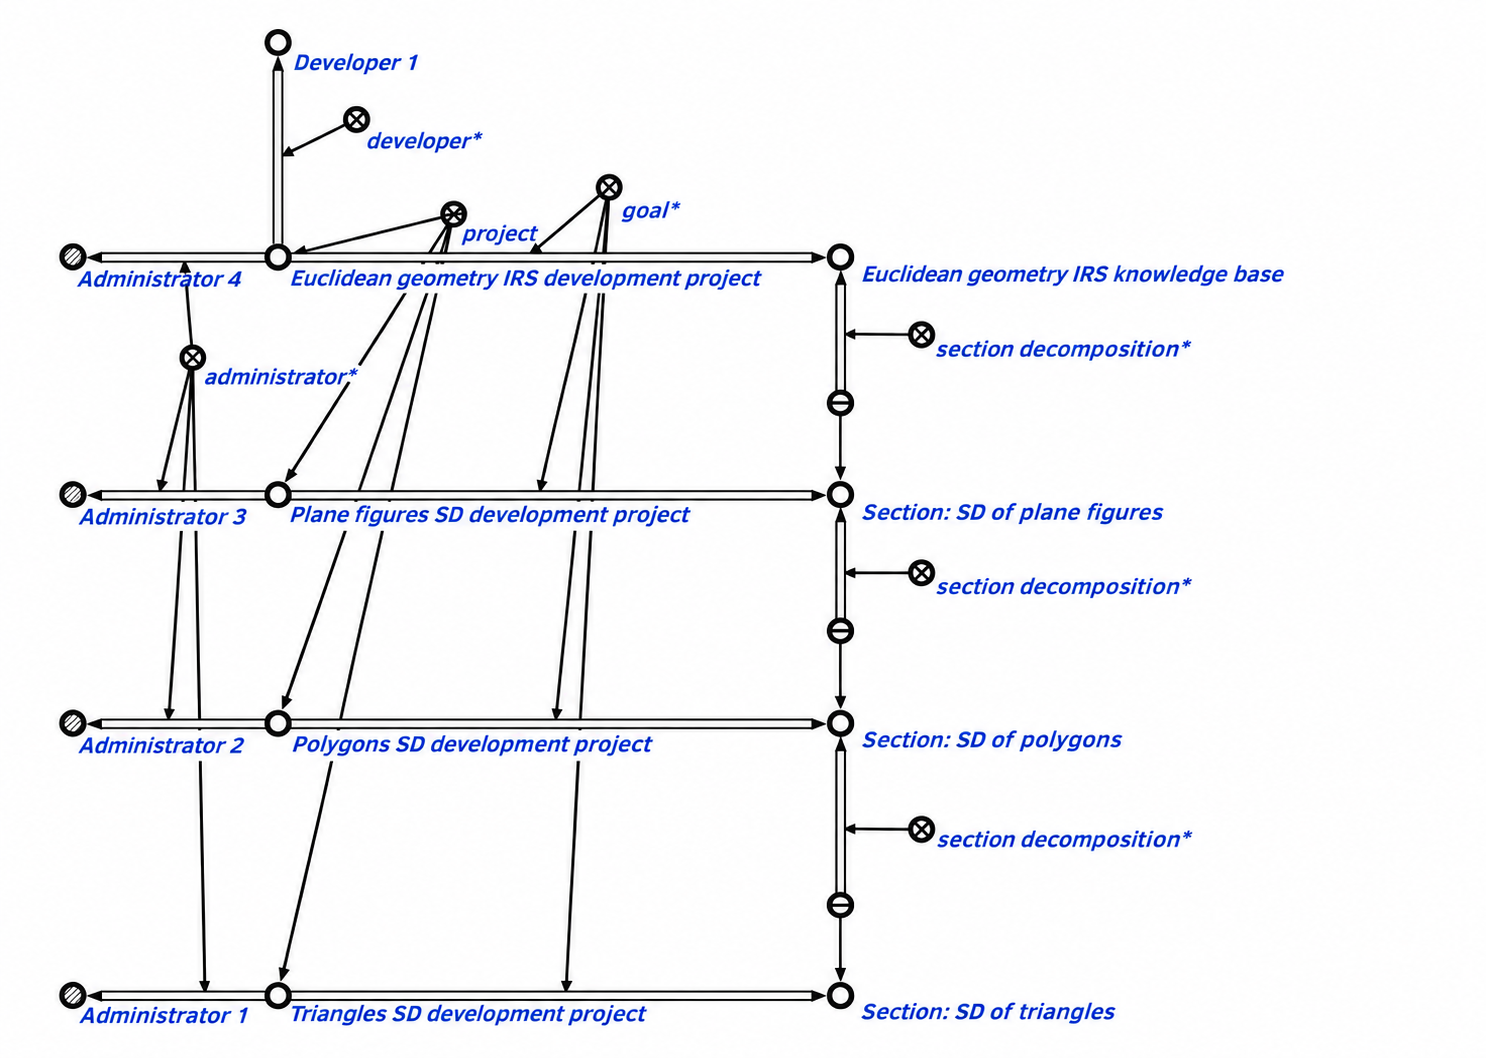
\includegraphics[width=\linewidth,height=0.67\textheight,keepaspectratio]{figures/sd_kb_develop_methods/hierarchy_en.png}
		\end{figure}
		{\footnotesize \textit{IRS} means intelligent reference system. \textit{SD} means subject domain.}
	\end{SCn}
\end{frame}

\begin{frame}{\\Manager role}
	\topline
	\justifying
	\begin{SCn}
		\scnheader{manager*}
		\scnidtf{binary relation linking a project to develop a section of an OSTIS knowledge base (or the entire knowledge base) to the sc-element denoting the person who manages that section}
	\end{SCn}
	\textbf{Manager responsibilities}
	\begin{textitemize}
		\item Plan the scope of knowledge base development work.
		\item Set priorities and deadlines.
		\item Define project tasks, break them down into subtasks, and assign them to developers.
		\item Track task deadlines.
	\end{textitemize}
\end{frame}

\begin{frame}{\\Expert role}
	\topline
	\justifying
	\begin{SCn}
		\scnheader{expert*}
		\scnidtf{binary relation linking a project to develop a section of an OSTIS knowledge base to the sc-element denoting the expert for that section}
	\end{SCn}
	\textbf{Expert responsibilities}
	\begin{textitemize}
		\item Verify the results of project tasks.
		\item Comment on the correctness of any knowledge base fragment. Any participant can also leave a natural-language comment on a fragment or element so that the group can discuss it. The system stores these comments in the \textit{current IS development} section.
	\end{textitemize}
\end{frame}

\begin{frame}{\\Access permissions by role}
	\topline
	\justifying
	\vspace{7mm}
	\begin{SCn}
		\begin{figure}[H]
			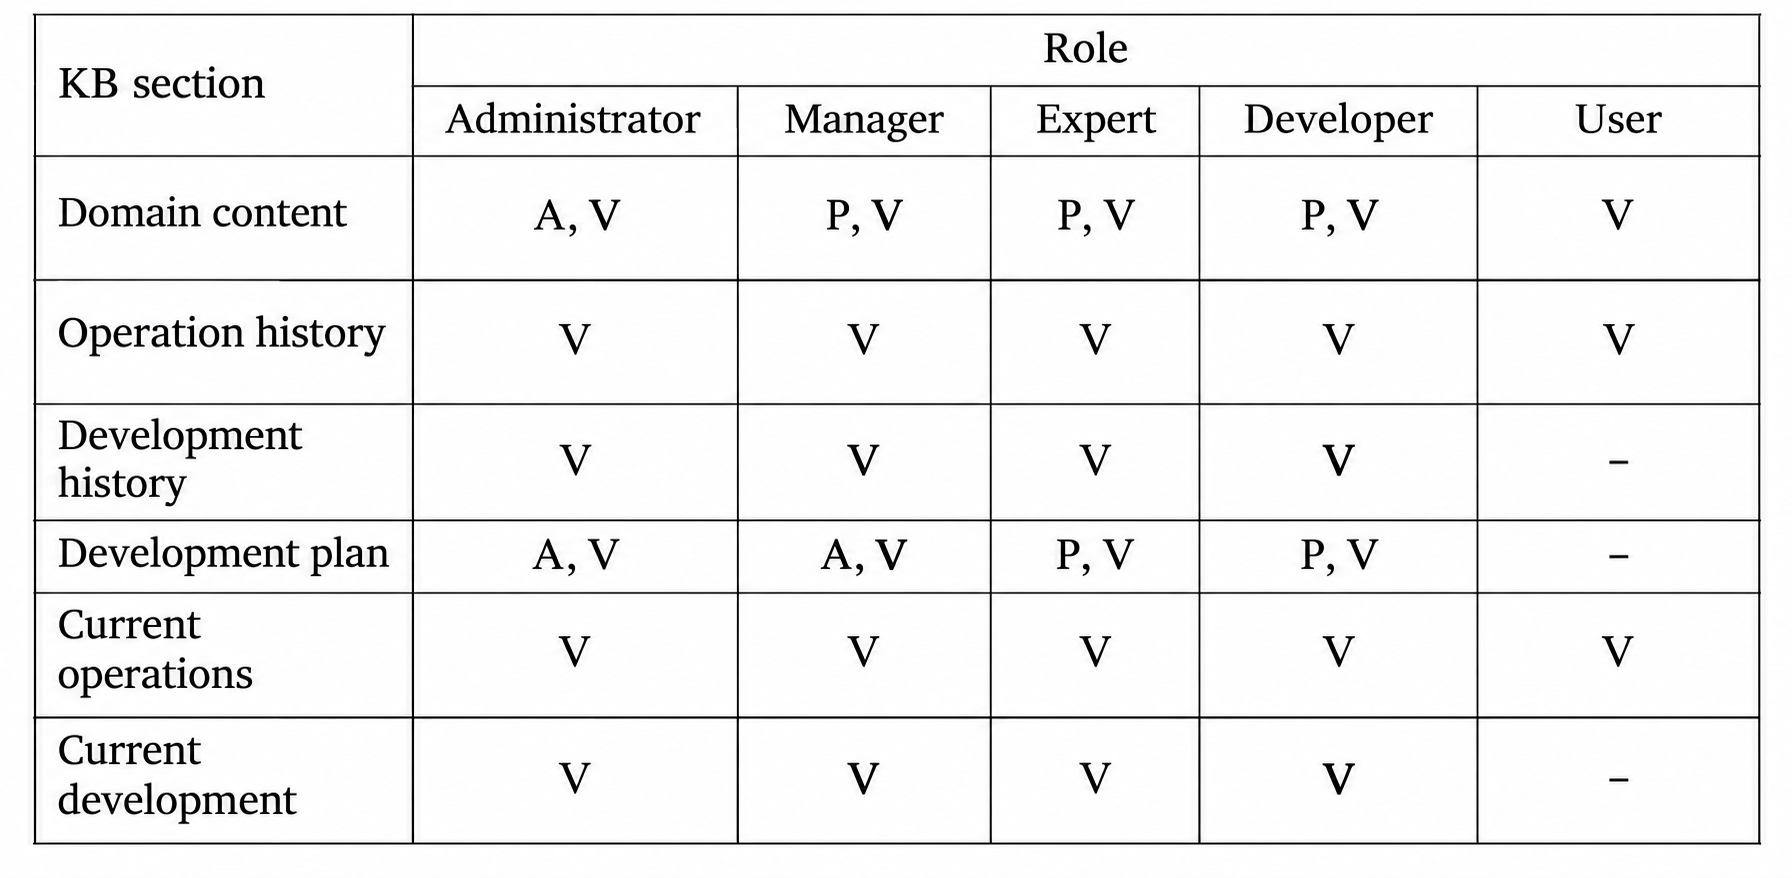
\includegraphics[width=\linewidth,height=0.72\textheight,keepaspectratio]{figures/sd_kb_develop_methods/table_en.png}
		\end{figure}
	\end{SCn}
\end{frame}

\begin{frame}{\\How to read the permissions table}
	\topline
	\justifying
	\begin{SCn}
		Each cell shows which permissions the role has for that section:
		\begin{textitemize}
			\item \textbf{P} means proposing edits.
			\item \textbf{V} means viewing the section.
			\item \textbf{A} means editing the section with automatic creation and acceptance of the corresponding proposal.
		\end{textitemize}
	\end{SCn}
\end{frame}

\begin{frame}{\\Knowledge base structure for developers}
	\topline
	\justifying
	\vspace{7mm}
	\begin{SCn}
		\begin{figure}[H]
			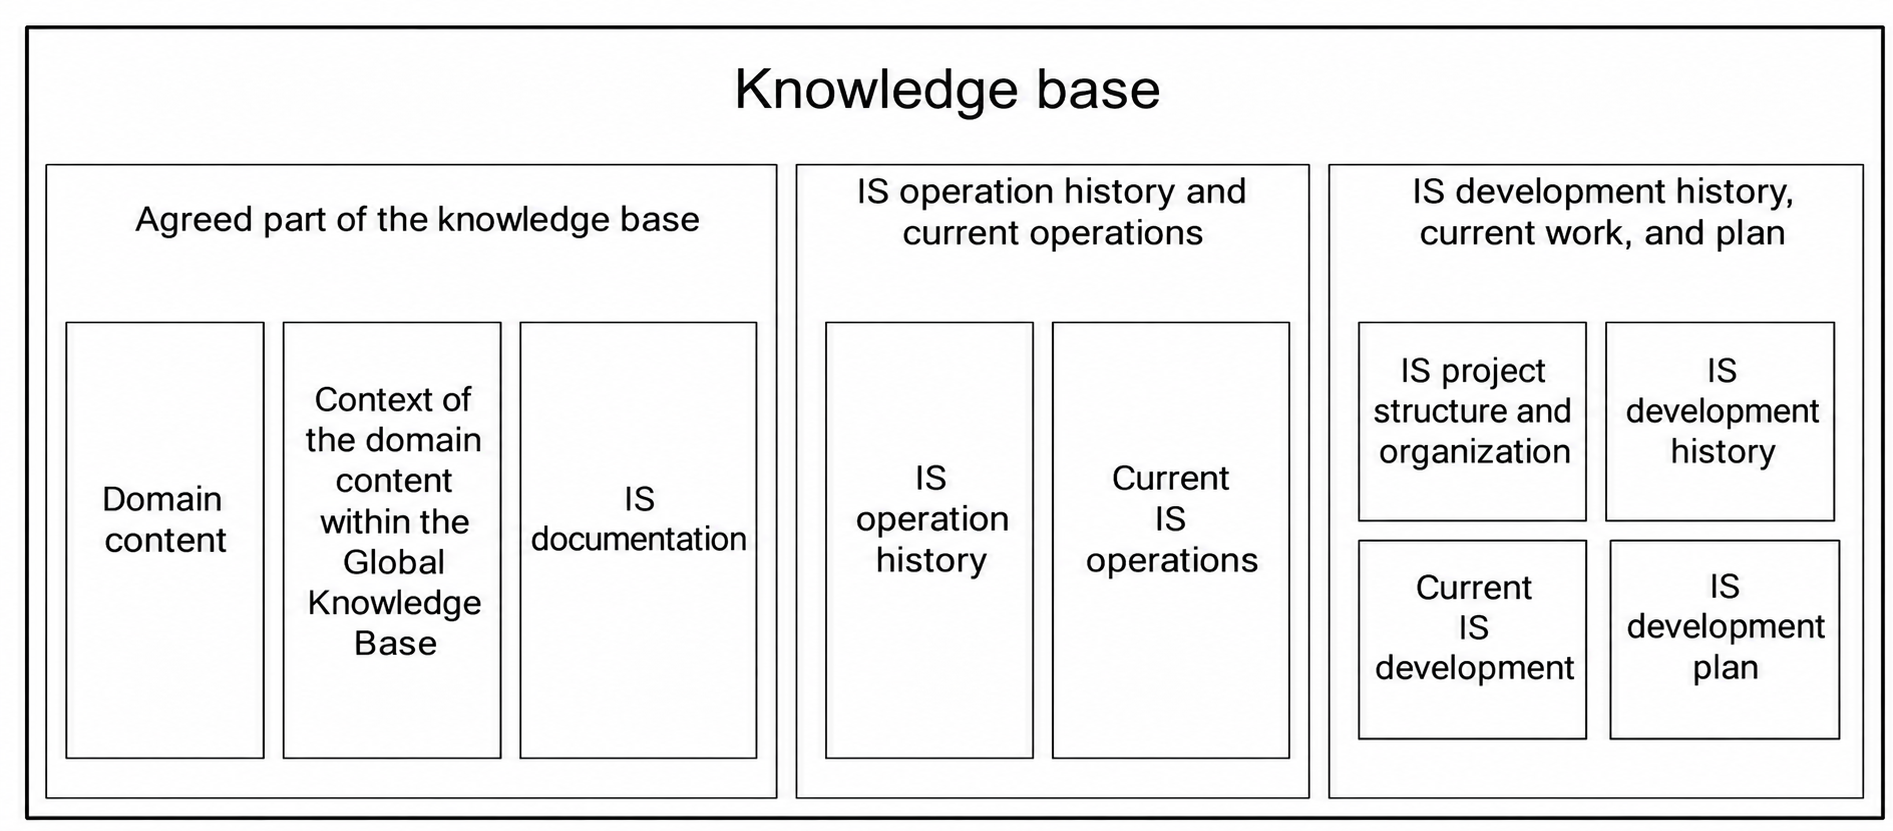
\includegraphics[width=\linewidth,height=0.70\textheight,keepaspectratio]{figures/sd_kb_develop_methods/kb_struct_develop_en.png}
		\end{figure}
	\end{SCn}
\end{frame}

\begin{frame}{\\Knowledge base structure for developers}
	\topline
	\justifying
	\begin{SCn}
		\scnheader{knowledge base}
		\begin{scnrelfromset}{partition}
			\scnitem{agreed part of the knowledge base}
			\scnitem{IS operation history and current operations}
			\scnitem{IS development history, current work, and plan}
		\end{scnrelfromset}
		\scntext{note}{A system that can evolve needs dedicated sections in its knowledge base. These sections record future development plans and current and past development work.}
	\end{SCn}
\end{frame}

\begin{frame}{\\Agreed part of the knowledge base}
	\topline
	\justifying
	\begin{SCn}
		\scnheader{agreed part of the knowledge base}
		\scnidtf{part of the knowledge base that all development participants currently agree on}
		\scnidtf{part of the knowledge base available to end users in operation mode}
		\scntext{note}{Distinguishing the agreed part allows the system to hide internal information unrelated to its operation from end users.}
	\end{SCn}
\end{frame}

\begin{frame}{\\Contents of the agreed part}
	\topline
	\justifying
	\vspace{5mm}
	\begin{SCn}
		\scnheader{agreed part of the knowledge base}
		\begin{scnrelfromset}{partition}
			\scnitem{domain content}
			\scnitem{context of the domain content within the Global Knowledge Base}
			\scnitem{IS documentation}
		\end{scnrelfromset}

		\scnheader{Global Knowledge Base}
		\scnidtf{global abstract semantic space of all knowledge accumulated by humanity to date}

		\scnheader{domain content}
		\scnidtf{part of the knowledge base containing all information about the subject domain (or several related subject domains) that the system is designed to work with}
	\end{SCn}
\end{frame}

\begin{frame}{\\Domain context and system documentation}
	\topline
	\justifying
	\begin{SCn}
		\scnheader{context of the domain content within the Global Knowledge Base}
		\scnidtf{specification of related objects that are mentioned when describing concepts under study, although they are not themselves studied in the domain content of the system's knowledge base}
		\scntext{example}{For a system dealing with Euclidean geometry, the context includes historical information about Euclid, his life, and mathematics.}

		\scnheader{computer system documentation}
		\scnidtf{OSTIS system documentation, including specifications of the knowledge base, knowledge processing machine, and interface, and guides for learning to use the system}
	\end{SCn}
\end{frame}

\begin{frame}{\\Operation history and current operations}
	\topline
	\justifying
	\begin{SCn}
		\scnheader{IS operation history and current operations}
		\begin{scnrelfromset}{partition}
			\scnitem{IS operation history}
			\scnitem{current IS operations}
		\end{scnrelfromset}

		\scnheader{IS operation history}
		\scnidtf{history of the system's dialogue with its users}
		\scnidtf{specification of all actions the system performed to meet users' information needs, including answers to questions and requested knowledge base transformations, along with their order and results}
	\end{SCn}
\end{frame}

\begin{frame}{\\Operation history and current operations}
	\topline
	\justifying
	\begin{SCn}
		\scnheader{IS operation history}
		\scntext{note}{Users can browse their past dialogue with the system. The system can analyze this information to adapt to how each user interacts with it.}

		\scnheader{current IS operations}
		\scnidtf{specifications of all actions the OSTIS system is currently performing, and all temporary auxiliary constructs generated by sc-agents that have yet to be removed}
		\scntext{note}{When these actions finish, their signs and specifications are moved to the system's operation history.}
	\end{SCn}
\end{frame}

\begin{frame}{\\Development history, work, and plan}
	\topline
	\justifying
	\begin{SCn}
		\scnheader{IS development history, current work, and plan}
		\begin{scnrelfromset}{partition}
			\scnitem{IS development history}
			\scnitem{IS development plan}
			\scnitem{IS project structure and organization}
			\scnitem{current IS development}
		\end{scnrelfromset}

		\scnheader{IS project structure and organization}
		\scnidtf{description of the project to develop the OSTIS system, including its subprojects and the roles of the developers responsible for each one}
	\end{SCn}
\end{frame}

\begin{frame}{\\Development history and current work}
	\topline
	\justifying
	\begin{SCn}
		\scnheader{IS development history}
		\scnidtf{specifications of project actions completed during development, recording who carried them out, their sequence, and their results}
		\scntext{explanation}{This information makes it possible to undo knowledge base changes and account for completed tasks when planning future work.}

		\scnheader{current IS development}
		\scnidtf{specifications of approved project actions that developers have started and are currently carrying out, including who is doing them, their sequence, and their purpose}
	\end{SCn}
\end{frame}

\begin{frame}{\\System development plan}
	\topline
	\justifying
	\begin{SCn}
		\scnheader{computer system development plan}
		\scnidtf{specifications of project actions approved for execution that are not yet under way, along with proposals to edit the section on development history, current work, and plans, and discussions of those proposals by administrators, managers, and experts}
	\end{SCn}
\end{frame}

\begin{frame}{\\Past and present states}
	\topline
	\justifying
	\begin{SCn}
		\scnheader{past state of the knowledge base}
		\begin{scnreltoset}{basic decomposition}
			\scnitem{IS development history}
			\scnitem{IS operation history}
		\end{scnreltoset}
		\scnheader{present state of the knowledge base}
		\begin{scnreltoset}{basic decomposition}
			\scnitem{current IS development}
			\scnitem{IS project structure and organization}
			\scnitem{agreed part of the knowledge base}
			\scnitem{current IS operations}
		\end{scnreltoset}
	\end{SCn}
\end{frame}

\begin{frame}{\\Future state}
	\topline
	\justifying
	\begin{SCn}
		\scnheader{future state of the knowledge base}
		\begin{scnreltoset}{basic decomposition}
			\scnitem{IS development plan}
			\scnitem{IS operation history}
		\end{scnreltoset}
	\end{SCn}
\end{frame}

\iffalse
\begin{frame}{Principles of collaboration among developers}% TODO
	\topline
	\justifying
	\begin{SCn}
	\end{SCn}
\end{frame}
\fi

\begin{frame}{\\Knowledge base verification}
	\topline
	\justifying
	\begin{SCn}
		\scnheader{knowledge base verification}
		\scnidtf{checking knowledge bases for problematic structures}
	\end{SCn}

	The following ontologies support the detection and correction of incomplete or incorrect knowledge and the removal of information clutter:
	\begin{textitemize}
		\item completeness ontologies that formally \textit{specify the completeness requirements} for representing the relevant subject domains in sc-memory
		\item ontologies that specify \textit{classes of constructs} that constitute errors or information clutter in the relevant subject domains
	\end{textitemize}
\end{frame}

\begin{frame}{\\Identifying problematic structures}
	\topline
	\justifying
	\vspace{5mm}

	Defining classes of problematic structures makes it possible to specify those structures for knowledge base developers and for agents to process automatically.

	By specifying problematic structures in its knowledge base, an intelligent system can \textit{analyze} its own knowledge for correctness, completeness, and redundancy and \textit{evaluate} the knowledge and skills it has acquired. This gives the system the ability to reflect on its own knowledge.

	\textbf{Types of problematic structures}
	\begin{textitemize}
		\item incorrect structures
		\item structures that describe incomplete knowledge
		\item information clutter
	\end{textitemize}
\end{frame}

\begin{frame}{\\Types of problematic structures}
	\topline
	\justifying
	\begin{SCn}
		\scnheader{incorrect structure}
		\scnidtf{structure containing a knowledge base fragment in which an error has been detected}

		\scnheader{structure that describes incomplete knowledge}
		\scnidtf{structure containing a knowledge base fragment that lacks information needed to understand its meaning fully and unambiguously}

		\scnheader{information clutter}
		\scnidtf{structure containing a knowledge base fragment that has become unnecessary and should be removed}
	\end{SCn}
\end{frame}

\begin{frame}{\\Examples of incomplete knowledge}
	\topline
	\justifying
	\vspace{7mm}

	A knowledge base can be incomplete in the following ways:
	\begin{textitemize}
		\item A given entity has main identifiers in only some of the external languages.
		\item A definition does not specify the constants it uses.
		\item A semantic neighborhood does not identify its key sc-element.
		\item A subject domain does not specify its maximal class of objects of study.
		\item A relation does not specify its domains.
		\item A measurable parameter has no unit or scale of measurement.
		\item A concept is not associated with any subject domain.
	\end{textitemize}
\end{frame}

\iffalse
\begin{frame}{\\Detecting incomplete knowledge}% TODO
	\topline
	\justifying
	\begin{SCn}
	\end{SCn}
\end{frame}
\fi
